\documentclass[a4paper,10pt]{article}
\usepackage[utf8]{inputenc}
\usepackage{graphicx,graphics} 
\usepackage{color}
\newcommand{\red}[1]{{\color{red} {#1}}}
\newcommand{\todo}[1]{{\color{red} TODO: {#1}}}
%opening

\title{Plan de thèse}
\author{Maël}
\graphicspath{{fig/}}
\begin{document}
 
\maketitle

\begin{abstract}
Voici mon plan de thèse.
\end{abstract}
\section{Introduction}
Résumé  de tout ce qu'on va dire dans la section 2, puis plan de la these, et explication de ce qu'on a fait par rapport au problème.

\section{Contexte}

\subsection{Reseau}

\subsubsection{What is 5G ?}
Telecoms networks are constantly evolving. Nowadays, a new technology is starting to be deployed in the territory: 5G.The term 5G gather a set of functional specifications. The organism that sets these specifications is the ITU (International Telecommunication Union). For several years, the ITU, more precisely the ITU-R (radiocommunication component of the ITU) has been working to determine the functional aspect that 5G must satisfy. Figure~\ref{fig:5gperf} from~\cite{5GACIA} illustrates some of those fonctional aspects: a bitrate up to 20Gbps, low end to end latencies down to 1ms (we are focusing on this aspect in this thesis), a better availability and reliablity, that means close to zero failure or packet loss, a better security in the communications, or an higher connection density, up to 1 million devices per $km^2$.

  \begin{figure}[h]
      \begin{center}
      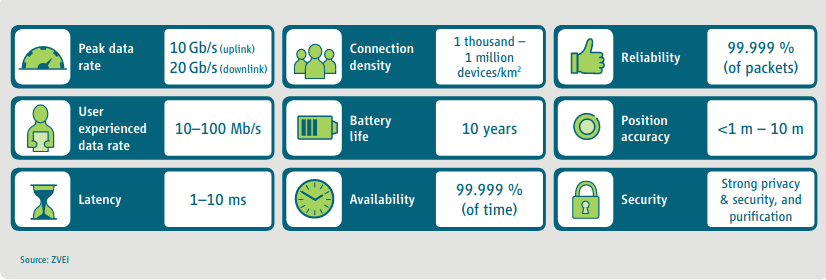
\includegraphics[width=1\textwidth]{performance5g.png}
      \end{center}
      \caption{5G performances required by ITU-R}\label{fig:5gperf}
      \end{figure}

All these aspects lead us to various application cases. Figure~\ref{fig:usecases} also taken from~\cite{5GACIA} establishes a non-exhaustive list of them, according to their different technical constraints. Indeed, low latency is required for applications like motion control that work in real time since one of the goals of 5G is to obtain dynamic programmable networks, for greater flexibility of use.
 In an other hand, an higher broadband aims applications like video streaming, augmented reality of ensuring the connectivity of a large number of terminals.
By relaxing latency and broadband constraints, it is possible to expand further the number of devices (up to 1 million) for applications like sensors networks.

  \begin{figure}[h] 
      \begin{center}
      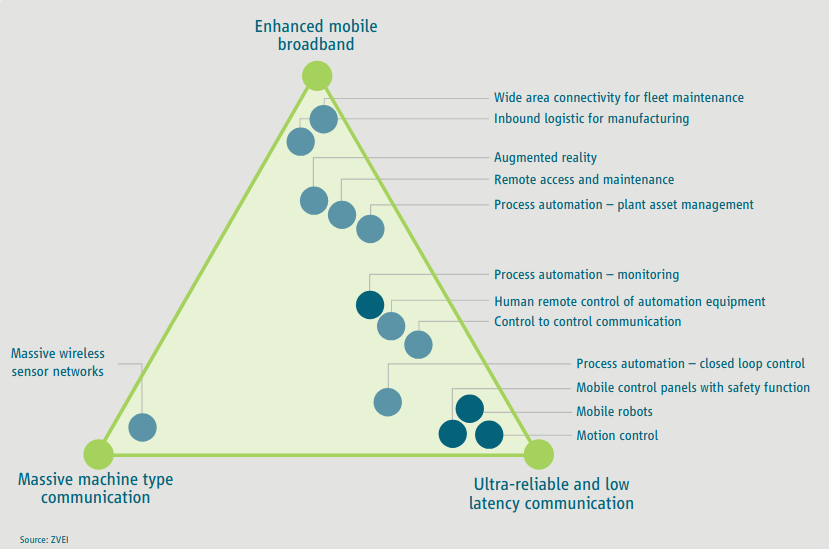
\includegraphics[width=1\textwidth]{usecases.png}
      \end{center}
      \caption{Some examples of use cases for 5G}\label{fig:usecases}
      \end{figure}
          


 All the requirements fixed by ITU-R are formally referenced in IMT-2020. \cite{dahlman20185g} is a good paper in which one can find all requirements of IMT-2020.
 

To meet these 5G functional specifications, the network equipments must follow some technical standards. 3GPP (3rd Generation Partnership Project) is an union between several standard organization which sets the technical specifications of 5G. 3GPP frequently publish some release, that regroup some new specifications. The first release focused on 5G was the release 15, released in 2018 \cite{RELEASENOKIA}.  

  \begin{figure}[h]
      \begin{center}
      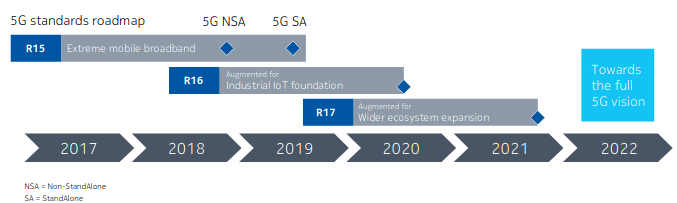
\includegraphics[width=1\textwidth]{release.png}
      \end{center}
      \caption{3GPP releases 15, 16 and 17 calendar}\label{fig:release}
      \end{figure}
  
Release 15 focused on increasing throughput and interworking between 4G and 5G, and introduced the notion of URLLC (Ultra-Reliable Low-Latency Communication). Release 16 an 17 deepened the notion of URLLC. The notion of URLLC consists in ensuring a low packet loss and a low latency communication. Indeed, several use cases (smart factories, control operations, ...) needs some highly reliable communications in which the latency must be bounded. Most of the current network does not ensure a bounded latency for all packets. This is why we talk about statistical multiplexing; the latency of a given network is, most of the time good, but the technology does not ensure a maximal latency for $100\%$ of the packets.  In this thesis, we focus on the low latency aspect of our communication. More precisely, URLLC aims to ensure a good end to end latency. To achieve such a goal, each component of the communication must meet the constraints, the radio communications, and the core network. This thesis focus on the core networks. 

\subsubsection{Cloud RAN}
Current mobile network (aka cellular network) architecture consists in a distributed radio access networks: the mobile terminals connect to base stations (BTS for Base Transceiver Station as a generic name, eNB for evolved Node B in 3GPP LTE “4G” standard) that encompasses all the sub-systems needed to realize mobile communication \cite{bouguen2012lte} It mainly comprises the radio part, that furnishes the connection between the mobile terminal and the BTS, and the network part that provides control and management functions like mobility support (the main functionality being the support of handover from one BTS to another, i.e. the ability to pursue a communication when moving from range of an antenna to another). The evolutions proposed in next generations aim at evolving toward centralized radio network architectures (C-RAN, for Cloud Radio Access Network) to reduce consumption costs and power at the base stations \cite{mobile2011c}. These C-RAN architectures include simplified base stations on the field. Depending on the architecture choice  
, it can be restricted to the radio part and the digital to analog conversion only. This can be identified by different names depending on the reference documents, including RU for Remote Unit or Remote Radio Heads (RRH). The later will be used the rest of the document. The other component of the C-RAN is composed of the processing units (baseband unit: BBU – used in this document – or FU for Frontend Unit) located in the cloud. By cloud we define in this document the capability of instantiating executable programs in data centers that are transparently connected to the systems requiring the results of the program execution. The execution may be indifferently performed on virtualized machines, or bare metal one, or any other combinations. The network between RRH and BBU is called “Fronthaul Network”, or “Fronthaul” for short. Figure~\ref{fig:fronthaul} illustrates an example of fronthaul in which several BBU are gathered in a same datacenter. 

  \begin{figure}[h]
      \begin{center}
      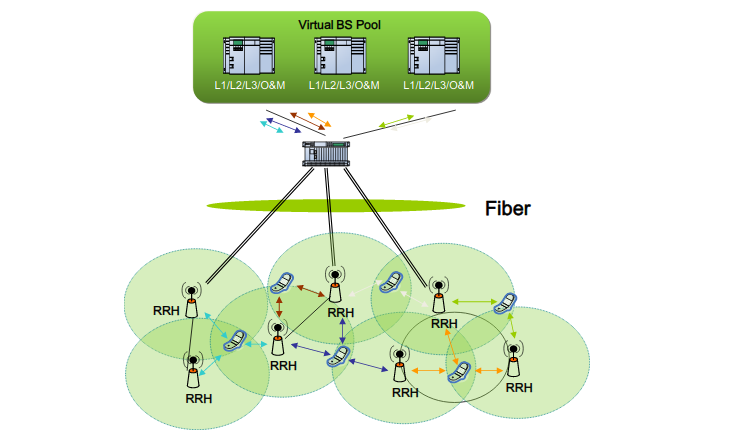
\includegraphics[width=1\textwidth]{fronthaul.png}
      \end{center}
      \caption{An example of fronthaul network for Clound RAN}\label{fig:fronthaul}
      \end{figure}
      
      Figure~\ref{fig:CRANsplit} illustrates the two different ways proposed to split the BTS. In the first one, called ``Full centralization'' the RRH integrates only the radio functions, while in the second one, called ``partial centralization'', the RRH keeps the baseband processing function. In the last case, the term BBU is not aporpriate anymore but is still used, in order to simplify the comprehension.
   \begin{figure}[h]
      \begin{center}
      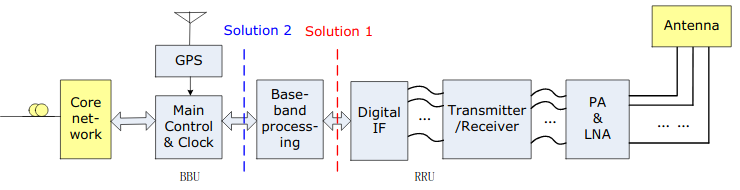
\includegraphics[width=1\textwidth]{CRANsplit.png}
      \end{center}
      \caption{The two different split for Cloud-RAN}\label{fig:CRANsplit}
      \end{figure}
       
This type of architecture faces the challenge of mastering the latency in the transfer process between the RRHs on the field and BBUs in the cloud. Low latency is already critical for the deployment of C-RAN approach in LTE “4G” networks. The standard requires hard time constraints for functions like HARQ (Hybrid Automatic Repeat reQuest) that needs to be processed in less than $3ms$ \cite{bouguen2012lte}. Considering processing time into the BBU, the time budget over the network can be as low as $400\mu s$ for a round trip. One specificity in this C-RAN context is not only the latency constraint, but also the periodicity of the data transfer between RRH and BBU (this HARQ constraint must be enforced for each frame emitted every millisecond). Looking beyond current mobile network generation, one must have in mind that ongoing 5G standards will require to reach end-to-end expected latency as low as $1ms$ (depending on targeted services) \cite{boccardi2014five}. New scheduling and new technologies have to be considered to guarantee delay constrained periodic data transfers. 


\subsubsection{Technical solution for low latency}


The expressed constraints expressed for C-RAN architecture and 5G standard are hardly met in current networks. In IP or even Ethernet networks, the traffic usually suffers of delay due to buffering. The amazing success of the packet based networks for the last 40 years relies on the statistical multiplexing: the packets are sent when they are ready and are buffered in intermediate nodes (routers for IP networks, switches for Ethernet networks) when contention arises \cite{venkatramani1994supporting}. A contention means that one resource (node out interface) is needed at the same time for transmission of several packets. In this case, the supplementary packets are stored in a buffer until the resources become available. This allows an easy deployment and management of a network, leading to a delivery of the packet with few loss (under conditions that buffers are big enough) but at the price of uncertainty on the delivery time. This uncontrolled and non predictable delay prevents to offer low latency and no jitter in the current network. Statistically managed QoS do not allow contention avoidance, then they can not provide null jitter \cite{khaunte2003technique}. If they can be used to prioritize some packets over the others (e.g. Express Forwarding against Best Effort), they fail to ensure delivery of a given packet in a given time delay when several packets compete for the same resource. 
The best current solution is to rely on an almost full optical approach, where each end-points (RRH on one side, BBU on the other side) are connected through direct fiber or full optical switches \cite{leclerc2016transmission}\cite{leclerc2016signaling}. This architecture is very expensive and hardly scales in the case of a mobile network. As illustrative purpose, a single (one operator) mobile network in France is composed of about $10,000$ base stations. This number will increase by a factor of $2$ to $20$ with the emergence of “small cells” that allow increasing base station density and to reach higher throughput \cite{leclerc2016transmission}\cite{leclerc2016signaling}. It is then needed to find a solution to offer low latency over commoditized packet based networks. 

Although 3GPP standards for 5G are not yet completely frozen, the core networks should use ethernet technology. Time Sensitive Networking (TSN) is a task group of IEEE that develop some standards in ethernet. The two standards we focus here are 802.1Qbu and 802.1Qbv \cite{ieee802}  
  
802.1Qbu allows frame preemption, that is, a node of the network is able to stop the transmission of a frame to send another frame. This brings us to a management of networks in which some flow can be considered as more critical than others. 

\todo{si on garde, schema + explications} 

802.1Qbv allows the nodes to manage different flows by a gate mechanism. Knowing the flows travelling over a node of the network, it is possible to schedule on an output port the time at which each flow must be sent by the node in order to prioritize the most critical flows. The scheduler sends a  GCL (gate control list) to the node. To one gate is associated one or several flows, and the nodes open or close the gates following the GCL.

Figure~\ref{fig:tsnqbv} found in \cite{durr2016no} shows the mechanism of a switch with the 802.1Qbv technology. Considering a given period ($T_{cycle}$ in the figure), the switch select at each times ($T_1 , T_2 , \ldots$ the queues that must be open to transmit packets. In figure 6, at time $T_1$, all gates exept the one for scheduled traffic are open, at time $T_2$, all gates are closed and at time $T_3$ only the gat for scheduled traffic is open.
  \begin{figure}[h]
      \begin{center}
      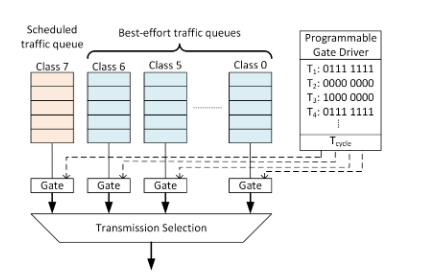
\includegraphics[width=0.8\textwidth]{tsnqbv.png}
      \end{center}
      \caption{IEEE 802.1Qbv mechanism}\label{fig:tsnqbv}
      \end{figure}

  
\subsection{Algo}
Expliquer ce qu'on a lu, pourquoi les models les plus proches sont différents, ou quelles sont les approches différentes que les gens ont eu. Ne pas trop rentrer dans les détails, on y reviendra notamment sur simons apres le problème

\section{Définition du problème}

\subsection{Model}
\begin{itemize}
 \item Temps discrets
 \item Description du routed network (modèle avec les sommets qui sont des conflits), Ce que ca réprésente en Cloud-RAN.
 \item Periodicité
 \item conflict depth
 
\end{itemize}
\subsection{Problèmes}
Definition de BRA,PALL, SPALL, Expliquer la différence entre les deux (exemple ou une solution optimale pour l'un ne l'est pas pour l'autre et inversement), les deux metriques sur chacuns des problèmes, et définition des problemes. NP-complétude pour chacun des problèmes, sur l'étoile ou en général.
Dire que PALL est moins contraint que SPALL.


\section{Flux désynchronisés}
Ne peux pas s'impliquer dans le contexte C-RAN, plus pour une 6G ou eventuellement on pourait désynchroniser les flux. Sinon dire que ca pourrait être utile dans un contexte différent (usine ou autre)
Dans cette section on ne s'interesse qu'a des flux désynchronisés dans une topologie en etoile.
On peut peut être simplifier le model, ou au moins les notations juste pour cette partie, car on a pas besoin  des buffers.
Justifier l'envie de ne rien buffuriser par l'utilisation des réseaux optiques.
\subsection{Flux desynchronisés sans buffer}
Définition du problème PAZL, variante de PALL dans laquelle on ne veux vraiment jamais buffuriser les messages.
Résultats théoriques interessants, mais non utilisable dans les autres parties, car vraiment sépcifiques au fait qu'on ne buffurise rien.\\
Courbes de résultats
\subsection{Flux desynch avec un seul buffer dans le datacenter}
Probleme PALL, explication qu'on découpe le probleme en aller/retour.
Au retour algo FPT basé du simons adapté pour la periodicité, a l'aller on a regardé ce que différents ordres donnaient.\\
Courbes de résultats
\section{Flux synchronisés}
Ici, on utilise des buffers dans le réseau. On a pas besoin de distinguer les différentes topologies, car les algos les resolvent toutes. \\
Rappeler les notions de conflict depth. dire qu'ici pour 1 c'est trivial et que apres nos algos s'adaptent a toutes les conflict depth, même si en pratique il vaut mieux qu'elle soit petite.
\subsection{Compact form}
Reprendre la définition de compact assignment etc
\subsection{Algorithms}
On a commencé par regarder différents algos greedy, rien ne sortait du lot.
Expliquer les différents algos de voisinage, tout ce qu'on a regardé dessus (tabou avec ou sans mémoire, Descente d'un point aléatoire ou non, Recuit avec ou sans descente avant, réglage parametres recuit...\\
Parler des coupes pour de l'algo branch and bound.\\
Courbes de résultats

\section{Gestion d'un second type de flux, BE}
Rappeler qu'il est possible avec TSN de mixer deux types de flux en gérant le traffic et donc en priorisant les flux CRAN. Le but de cette section est de montrer l'impact sur le best effort.

\subsection{BE dans les reseaux non optiques}
Dire que dans un cas plus général, on à pas ce changement de support qui rend l'organisation des flux facile. On peut néanmoins adapter le model en agrandissant la taille des paquets pour faire passer du best effort dedans. Regarder, cette derniere idée contre le fait de ne rien faire de particulier.
\subsection{travaux n-GREEN}
Parler pour introduire du prototype de dominique C
Expliquer en quoi la technologie fait qu'il est trivial d'organiser les flux C-RAN entre eux pour qu'il n'y ait pas de contention. 
Dire que du coup on essaye de les organiser pour impacter au moins le best effort. Résultat, le best effort est même avantagé.
\section{Adaptation industrielle}
\subsection{Onos}
Présentation de ONOS, TSN et de FPGA. Description de ce qu'olivier à programmé sur ONOS, du switch FPGA de brice et de comment on connecte tout ça. 

\section{Ouverture, conclusion}

\subsection{Reinforcement learning}
\subsection{Model plus large avec tout ce qu'on a pas utilisé}
-Liens de vitesse différentes, tailles de paquets différents...
\subsection{questions ouvertes / suite de la these}

\bibliographystyle{ieeetr}
\bibliography{src}
\end{document}
